
%% bare_jrnl_compsoc.tex
%% V1.4b
%% 2015/08/26
%% by Michael Shell
%% See:
%% http://www.michaelshell.org/
%% for current contact information.
%%
%% This is a skeleton file demonstrating the use of IEEEtran.cls
%% (requires IEEEtran.cls version 1.8b or later) with an IEEE
%% Computer Society journal paper.
%%
%% Support sites:
%% http://www.michaelshell.org/tex/ieeetran/
%% http://www.ctan.org/pkg/ieeetran
%% and
%% http://www.ieee.org/

%%*************************************************************************
%% Legal Notice:
%% This code is offered as-is without any warranty either expressed or
%% implied; without even the implied warranty of MERCHANTABILITY or
%% FITNESS FOR A PARTICULAR PURPOSE!
%% User assumes all risk.
%% In no event shall the IEEE or any contributor to this code be liable for
%% any damages or losses, including, but not limited to, incidental,
%% consequential, or any other damages, resulting from the use or misuse
%% of any information contained here.
%%
%% All comments are the opinions of their respective authors and are not
%% necessarily endorsed by the IEEE.
%%
%% This work is distributed under the LaTeX Project Public License (LPPL)
%% ( http://www.latex-project.org/ ) version 1.3, and may be freely used,
%% distributed and modified. A copy of the LPPL, version 1.3, is included
%% in the base LaTeX documentation of all distributions of LaTeX released
%% 2003/12/01 or later.
%% Retain all contribution notices and credits.
%% ** Modified files should be clearly indicated as such, including  **
%% ** renaming them and changing author support contact information. **
%%*************************************************************************

% *** Authors should verify (and, if needed, correct) their LaTeX system  ***
% *** with the testflow diagnostic prior to trusting their LaTeX platform ***
% *** with production work. The IEEE's font choices and paper sizes can   ***
% *** trigger bugs that do not appear when using other class files.       ***                          ***
% The testflow support page is at:
% http://www.michaelshell.org/tex/testflow/

\documentclass[10pt,journal,compsoc]{IEEEtran}
%
% If IEEEtran.cls has not been installed into the LaTeX system files,
% manually specify the path to it like:
% \documentclass[10pt,journal,compsoc]{../sty/IEEEtran}

% Some very useful LaTeX packages include:
% (uncomment the ones you want to load)

% *** MISC UTILITY PACKAGES ***
%
%\usepackage{ifpdf}
% Heiko Oberdiek's ifpdf.sty is very useful if you need conditional
% compilation based on whether the output is pdf or dvi.
% usage:
% \ifpdf
%   % pdf code
% \else
%   % dvi code
% \fi
% The latest version of ifpdf.sty can be obtained from:
% http://www.ctan.org/pkg/ifpdf
% Also, note that IEEEtran.cls V1.7 and later provides a builtin
% \ifCLASSINFOpdf conditional that works the same way.
% When switching from latex to pdflatex and vice-versa, the compiler may
% have to be run twice to clear warning/error messages.

% *** CITATION PACKAGES ***
%
\ifCLASSOPTIONcompsoc
  % IEEE Computer Society needs nocompress option
  % requires cite.sty v4.0 or later (November 2003)
    \usepackage[nocompress]{cite}
\usepackage{amsmath}
\usepackage{graphicx}
%\usepackage{verbatim}  %add multiple lines of comments
%\usepackage{marvosym}  %add the \Letter command
%\usepackage{euscript}
%\usepackage{wasysym}
%\usepackage{mathrsfs}

\else
  % normal IEEE
  \usepackage{cite}
\fi
% cite.sty was written by Donald Arseneau
% V1.6 and later of IEEEtran pre-defines the format of the cite.sty package
% \cite{} output to follow that of the IEEE. Loading the cite package will
% result in citation numbers being automatically sorted and properly
% "compressed/ranged". e.g., [1], [9], [2], [7], [5], [6] without using
% cite.sty will become [1], [2], [5]--[7], [9] using cite.sty. cite.sty's
% \cite will automatically add leading space, if needed. Use cite.sty's
% noadjust option (cite.sty V3.8 and later) if you want to turn this off
% such as if a citation ever needs to be enclosed in parenthesis.
% cite.sty is already installed on most LaTeX systems. Be sure and use
% version 5.0 (2009-03-20) and later if using hyperref.sty.
% The latest version can be obtained at:
% http://www.ctan.org/pkg/cite
% The documentation is contained in the cite.sty file itself.
%
% Note that some packages require special options to format as the Computer
% Society requires. In particular, Computer Society  papers do not use
% compressed citation ranges as is done in typical IEEE papers
% (e.g., [1]-[4]). Instead, they list every citation separately in order
% (e.g., [1], [2], [3], [4]). To get the latter we need to load the cite
% package with the nocompress option which is supported by cite.sty v4.0
% and later. Note also the use of a CLASSOPTION conditional provided by
% IEEEtran.cls V1.7 and later.

% *** GRAPHICS RELATED PACKAGES ***
%
\ifCLASSINFOpdf
  % \usepackage[pdftex]{graphicx}
  % declare the path(s) where your graphic files are
  % \graphicspath{{../pdf/}{../jpeg/}}
  % and their extensions so you won't have to specify these with
  % every instance of \includegraphics
  % \DeclareGraphicsExtensions{.pdf,.jpeg,.png}
\else
  % or other class option (dvipsone, dvipdf, if not using dvips). graphicx
  % will default to the driver specified in the system graphics.cfg if no
  % driver is specified.
  % \usepackage[dvips]{graphicx}
  % declare the path(s) where your graphic files are
  % \graphicspath{{../eps/}}
  % and their extensions so you won't have to specify these with
  % every instance of \includegraphics
  % \DeclareGraphicsExtensions{.eps}
\fi
% graphicx was written by David Carlisle and Sebastian Rahtz. It is
% required if you want graphics, photos, etc. graphicx.sty is already
% installed on most LaTeX systems. The latest version and documentation
% can be obtained at:
% http://www.ctan.org/pkg/graphicx
% Another good source of documentation is "Using Imported Graphics in
% LaTeX2e" by Keith Reckdahl which can be found at:
% http://www.ctan.org/pkg/epslatex
%
% latex, and pdflatex in dvi mode, support graphics in encapsulated
% postscript (.eps) format. pdflatex in pdf mode supports graphics
% in .pdf, .jpeg, .png and .mps (metapost) formats. Users should ensure
% that all non-photo figures use a vector format (.eps, .pdf, .mps) and
% not a bitmapped formats (.jpeg, .png). The IEEE frowns on bitmapped formats
% which can result in "jaggedy"/blurry rendering of lines and letters as
% well as large increases in file sizes.
%
% You can find documentation about the pdfTeX application at:
% http://www.tug.org/applications/pdftex

% *** MATH PACKAGES ***
%
%\usepackage{amsmath}
% A popular package from the American Mathematical Society that provides
% many useful and powerful commands for dealing with mathematics.
%
% Note that the amsmath package sets \interdisplaylinepenalty to 10000
% thus preventing page breaks from occurring within multiline equations. Use:
%\interdisplaylinepenalty=2500
% after loading amsmath to restore such page breaks as IEEEtran.cls normally
% does. amsmath.sty is already installed on most LaTeX systems. The latest
% version and documentation can be obtained at:
% http://www.ctan.org/pkg/amsmath

% *** SPECIALIZED LIST PACKAGES ***
%
%\usepackage{algorithmic}
% algorithmic.sty was written by Peter Williams and Rogerio Brito.
% This package provides an algorithmic environment fo describing algorithms.
% You can use the algorithmic environment in-text or within a figure
% environment to provide for a floating algorithm. Do NOT use the algorithm
% floating environment provided by algorithm.sty (by the same authors) or
% algorithm2e.sty (by Christophe Fiorio) as the IEEE does not use dedicated
% algorithm float types and packages that provide these will not provide
% correct IEEE style captions. The latest version and documentation of
% algorithmic.sty can be obtained at:
% http://www.ctan.org/pkg/algorithms
% Also of interest may be the (relatively newer and more customizable)
% algorithmicx.sty package by Szasz Janos:
% http://www.ctan.org/pkg/algorithmicx

% *** ALIGNMENT PACKAGES ***
%
%\usepackage{array}
% Frank Mittelbach's and David Carlisle's array.sty patches and improves
% the standard LaTeX2e array and tabular environments to provide better
% appearance and additional user controls. As the default LaTeX2e table
% generation code is lacking to the point of almost being broken with
% respect to the quality of the end results, all users are strongly
% advised to use an enhanced (at the very least that provided by array.sty)
% set of table tools. array.sty is already installed on most systems. The
% latest version and documentation can be obtained at:
% http://www.ctan.org/pkg/array

% IEEEtran contains the IEEEeqnarray family of commands that can be used to
% generate multiline equations as well as matrices, tables, etc., of high
% quality.

% *** SUBFIGURE PACKAGES ***
%\ifCLASSOPTIONcompsoc
%  \usepackage[caption=false,font=footnotesize,labelfont=sf,textfont=sf]{subfig}
%\else
%  \usepackage[caption=false,font=footnotesize]{subfig}
%\fi
% subfig.sty, written by Steven Douglas Cochran, is the modern replacement
% for subfigure.sty, the latter of which is no longer maintained and is
% incompatible with some LaTeX packages including fixltx2e. However,
% subfig.sty requires and automatically loads Axel Sommerfeldt's caption.sty
% which will override IEEEtran.cls' handling of captions and this will result
% in non-IEEE style figure/table captions. To prevent this problem, be sure
% and invoke subfig.sty's "caption=false" package option (available since
% subfig.sty version 1.3, 2005/06/28) as this is will preserve IEEEtran.cls
% handling of captions.
% Note that the Computer Society format requires a sans serif font rather
% than the serif font used in traditional IEEE formatting and thus the need
% to invoke different subfig.sty package options depending on whether
% compsoc mode has been enabled.
%
% The latest version and documentation of subfig.sty can be obtained at:
% http://www.ctan.org/pkg/subfig

% *** FLOAT PACKAGES ***
%
%\usepackage{fixltx2e}
% fixltx2e, the successor to the earlier fix2col.sty, was written by
% Frank Mittelbach and David Carlisle. This package corrects a few problems
% in the LaTeX2e kernel, the most notable of which is that in current
% LaTeX2e releases, the ordering of single and double column floats is not
% guaranteed to be preserved. Thus, an unpatched LaTeX2e can allow a
% single column figure to be placed prior to an earlier double column
% figure.
% Be aware that LaTeX2e kernels dated 2015 and later have fixltx2e.sty's
% corrections already built into the system in which case a warning will
% be issued if an attempt is made to load fixltx2e.sty as it is no longer
% needed.
% The latest version and documentation can be found at:
% http://www.ctan.org/pkg/fixltx2e

%\usepackage{stfloats}
% stfloats.sty was written by Sigitas Tolusis. This package gives LaTeX2e
% the ability to do double column floats at the bottom of the page as well
% as the top. (e.g., "\begin{figure*}[!b]" is not normally possible in
% LaTeX2e). It also provides a command:
%\fnbelowfloat
% to enable the placement of footnotes below bottom floats (the standard
% LaTeX2e kernel puts them above bottom floats). This is an invasive package
% which rewrites many portions of the LaTeX2e float routines. It may not work
% with other packages that modify the LaTeX2e float routines. The latest
% version and documentation can be obtained at:
% http://www.ctan.org/pkg/stfloats
% Do not use the stfloats baselinefloat ability as the IEEE does not allow
% \baselineskip to stretch. Authors submitting work to the IEEE should note
% that the IEEE rarely uses double column equations and that authors should try
% to avoid such use. Do not be tempted to use the cuted.sty or midfloat.sty
% packages (also by Sigitas Tolusis) as the IEEE does not format its papers in
% such ways.
% Do not attempt to use stfloats with fixltx2e as they are incompatible.
% Instead, use Morten Hogholm'a dblfloatfix which combines the features
% of both fixltx2e and stfloats:
%
% \usepackage{dblfloatfix}
% The latest version can be found at:
% http://www.ctan.org/pkg/dblfloatfix

%\ifCLASSOPTIONcaptionsoff
%  \usepackage[nomarkers]{endfloat}
% \let\MYoriglatexcaption\caption
% \renewcommand{\caption}[2][\relax]{\MYoriglatexcaption[#2]{#2}}
%\fi
% endfloat.sty was written by James Darrell McCauley, Jeff Goldberg and
% Axel Sommerfeldt. This package may be useful when used in conjunction with
% IEEEtran.cls'  captionsoff option. Some IEEE journals/societies require that
% submissions have lists of figures/tables at the end of the paper and that
% figures/tables without any captions are placed on a page by themselves at
% the end of the document. If needed, the draftcls IEEEtran class option or
% \CLASSINPUTbaselinestretch interface can be used to increase the line
% spacing as well. Be sure and use the nomarkers option of endfloat to
% prevent endfloat from "marking" where the figures would have been placed
% in the text. The two hack lines of code above are a slight modification of
% that suggested by in the endfloat docs (section 8.4.1) to ensure that
% the full captions always appear in the list of figures/tables - even if
% the user used the short optional argument of \caption[]{}.
% IEEE papers do not typically make use of \caption[]'s optional argument,
% so this should not be an issue. A similar trick can be used to disable
% captions of packages such as subfig.sty that lack options to turn off
% the subcaptions:
% For subfig.sty:
% \let\MYorigsubfloat\subfloat
% \renewcommand{\subfloat}[2][\relax]{\MYorigsubfloat[]{#2}}
% However, the above trick will not work if both optional arguments of
% the \subfloat command are used. Furthermore, there needs to be a
% description of each subfigure *somewhere* and endfloat does not add
% subfigure captions to its list of figures. Thus, the best approach is to
% avoid the use of subfigure captions (many IEEE journals avoid them anyway)
% and instead reference/explain all the subfigures within the main caption.
% The latest version of endfloat.sty and its documentation can obtained at:
% http://www.ctan.org/pkg/endfloat
%
% The IEEEtran \ifCLASSOPTIONcaptionsoff conditional can also be used
% later in the document, say, to conditionally put the References on a
% page by themselves.

% *** PDF, URL AND HYPERLINK PACKAGES ***
%
%\usepackage{url}
% url.sty was written by Donald Arseneau. It provides better support for
% handling and breaking URLs. url.sty is already installed on most LaTeX
% systems. The latest version and documentation can be obtained at:
% http://www.ctan.org/pkg/url
% Basically, \url{my_url_here}.

% *** Do not adjust lengths that control margins, column widths, etc. ***
% *** Do not use packages that alter fonts (such as pslatex).         ***
% There should be no need to do such things with IEEEtran.cls V1.6 and later.
% (Unless specifically asked to do so by the journal or conference you plan
% to submit to, of course. )

% correct bad hyphenation here
\hyphenation{op-tical net-works semi-conduc-tor}

\begin{document}
%
% paper title
% Titles are generally capitalized except for words such as a, an, and, as,
% at, but, by, for, in, nor, of, on, or, the, to and up, which are usually
% not capitalized unless they are the first or last word of the title.
% Linebreaks \\ can be used within to get better formatting as desired.
% Do not put math or special symbols in the title.
\title{Flexible Representation and Manipulation\\of Audio Signals on Quantum Computers}
%\title{FRQA: A flexible representation of quantum audio}
%
% author names and IEEE memberships
% note positions of commas and nonbreaking spaces ( ~ ) LaTeX will not break
% a structure at a ~ so this keeps an author's name from being broken across
% two lines.
% use \thanks{} to gain access to the first footnote area
% a separate \thanks must be used for each paragraph as LaTeX2e's \thanks
% was not built to handle multiple paragraphs
%
%\IEEEcompsocitemizethanks is a special \thanks that produces the bulleted
% lists the Computer Society journals use for "first footnote" author
% affiliations. Use \IEEEcompsocthanksitem which works much like \item
% for each affiliation group. When not in compsoc mode,
% \IEEEcompsocitemizethanks becomes like \thanks and
% \IEEEcompsocthanksitem becomes a line break with idention. This
% facilitates dual compilation, although admittedly the differences in the
% desired content of \author between the different types of papers makes a
% one-size-fits-all approach a daunting prospect. For instance, compsoc
% journal papers have the author affiliations above the "Manuscript
% received ..."  text while in non-compsoc journals this is reversed. Sigh.

\author{Fei~Yan, %~\IEEEmembership{Member,~IEEE,}
        Yiming~Guo, %~\IEEEmembership{Fellow,~OSA,}
        Abdullah~M.~Iliyasu, %~\IEEEmembership{Fellow,~OSA,}
        and~Huamin~Yang%~\IEEEmembership{Life~Fellow,~IEEE}% <-this % stops a space
\IEEEcompsocitemizethanks{\IEEEcompsocthanksitem F. Yan, Y. Guo, and H. Yang are with School of Computer Science and Technology, Changchun University of Science and Technology, No. 7089, Weixing Road, Changchun 130022, China. E-mail: yanfei@cust.edu.cn\protect\\
% note need leading \protect in front of \\ to get a newline within \thanks as
% \\ is fragile and will error, could use \hfil\break instead.
\IEEEcompsocthanksitem A. M. Iliyasu is with Electrical Engineering Department, College of Engineering, Prince Sattam Bin Abdulaziz University, Al-Kharj 11942, Kingdom of Saudi Arabia.}% <-this % stops an unwanted space
\thanks{}}

% note the % following the last \IEEEmembership and also \thanks -
% these prevent an unwanted space from occurring between the last author name
% and the end of the author line. i.e., if you had this:
%
% \author{....lastname \thanks{...} \thanks{...} }
%                     ^------------^------------^----Do not want these spaces!
%
% a space would be appended to the last name and could cause every name on that
% line to be shifted left slightly. This is one of those "LaTeX things". For
% instance, "\textbf{A} \textbf{B}" will typeset as "A B" not "AB". To get
% "AB" then you have to do: "\textbf{A}\textbf{B}"
% \thanks is no different in this regard, so shield the last } of each \thanks
% that ends a line with a % and do not let a space in before the next \thanks.
% Spaces after \IEEEmembership other than the last one are OK (and needed) as
% you are supposed to have spaces between the names. For what it is worth,
% this is a minor point as most people would not even notice if the said evil
% space somehow managed to creep in.

% The paper headers
\markboth{}%
{Shell \MakeLowercase{\textit{et al.}}: Bare Demo of IEEEtran.cls for Computer Society Journals}
% The only time the second header will appear is for the odd numbered pages
% after the title page when using the twoside option.
%
% *** Note that you probably will NOT want to include the author's ***
% *** name in the headers of peer review papers.                   ***
% You can use \ifCLASSOPTIONpeerreview for conditional compilation here if
% you desire.

% The publisher's ID mark at the bottom of the page is less important with
% Computer Society journal papers as those publications place the marks
% outside of the main text columns and, therefore, unlike regular IEEE
% journals, the available text space is not reduced by their presence.
% If you want to put a publisher's ID mark on the page you can do it like
% this:
%\IEEEpubid{0000--0000/00\$00.00~\copyright~2015 IEEE}
% or like this to get the Computer Society new two part style.
%\IEEEpubid{\makebox[\columnwidth]{\hfill 0000--0000/00/\$00.00~\copyright~2015 IEEE}%
%\hspace{\columnsep}\makebox[\columnwidth]{Published by the IEEE Computer Society\hfill}}
% Remember, if you use this you must call \IEEEpubidadjcol in the second
% column for its text to clear the IEEEpubid mark (Computer Society jorunal
% papers don't need this extra clearance.)

% use for special paper notices
%\IEEEspecialpapernotice{(Invited Paper)}

% for Computer Society papers, we must declare the abstract and index terms
% PRIOR to the title within the \IEEEtitleabstractindextext IEEEtran
% command as these need to go into the title area created by \maketitle.
% As a general rule, do not put math, special symbols or citations
% in the abstract or keywords.
\IEEEtitleabstractindextext{%
\begin{abstract}
  By analyzing the numerical representation of amplitude values in audio signals and integrating the time component, a representation for audio signals on quantum computers, FRQA, is proposed. The FRQA representation is a normalized state that facilitates basic audio signal operations targeting these parameters. The preparation and retrieval for FRQA are discussed and, based on the FRQA state, we realize the circuits to accomplish basic audio signal operations such as signal addition, signal inversion, signal delay, and signal reversal. These operations can be employed as the major components to build advanced operations for particular applications in the quantum computing domain.
\end{abstract}

% Note that keywords are not normally used for peerreview papers.
\begin{IEEEkeywords}
Quantum computing, quantum audio, audio representation, audio manipulation.
\end{IEEEkeywords}}

% make the title area
\maketitle

% To allow for easy dual compilation without having to reenter the
% abstract/keywords data, the \IEEEtitleabstractindextext text will
% not be used in maketitle, but will appear (i.e., to be "transported")
% here as \IEEEdisplaynontitleabstractindextext when the compsoc
% or transmag modes are not selected <OR> if conference mode is selected
% - because all conference papers position the abstract like regular
% papers do.
\IEEEdisplaynontitleabstractindextext
% \IEEEdisplaynontitleabstractindextext has no effect when using
% compsoc or transmag under a non-conference mode.

% For peer review papers, you can put extra information on the cover
% page as needed:
% \ifCLASSOPTIONpeerreview
% \begin{center} \bfseries EDICS Category: 3-BBND \end{center}
% \fi
%
% For peerreview papers, this IEEEtran command inserts a page break and
% creates the second title. It will be ignored for other modes.
\IEEEpeerreviewmaketitle

\IEEEraisesectionheading{\section{Introduction}\label{sec1}}
% Computer Society journal (but not conference!) papers do something unusual
% with the very first section heading (almost always called "Introduction").
% They place it ABOVE the main text! IEEEtran.cls does not automatically do
% this for you, but you can achieve this effect with the provided
% \IEEEraisesectionheading{} command. Note the need to keep any \label that
% is to refer to the section immediately after \section in the above as
% \IEEEraisesectionheading puts \section within a raised box.

% The very first letter is a 2 line initial drop letter followed
% by the rest of the first word in caps (small caps for compsoc).
%
% form to use if the first word consists of a single letter:
% \IEEEPARstart{A}{demo} file is ....
%
% form to use if you need the single drop letter followed by
% normal text (unknown if ever used by the IEEE):
% \IEEEPARstart{A}{}demo file is ....
%
% Some journals put the first two words in caps:
% \IEEEPARstart{T}{his demo} file is ....
%
% Here we have the typical use of a "T" for an initial drop letter
% and "HIS" in caps to complete the first word.
\IEEEPARstart{Q}{uantum} computation and quantum information, an area of study focused on accomplishing information processing tasks on quantum mechanical systems, has become a rapidly growing field since Feynman proposed the quantum computation model in 1982 \cite{1}. Afterwards, further developments by a number of researchers, notably, Deutsch's quantum parallelism assertion \cite{2}, Shor's integer factoring algorithm \cite{3}, and Grover's database searching algorithm \cite{4}, marked a leap forward in terms of the anticipated computing capability and secure communication for quantum computing devices. Not surprisingly, the appeal of this novel computational paradigm has continued to increase especially from scientists and engineers who work in areas related to this.

An image is a common artifact that depicts visual perception, which makes its realization and handling on the quantum computing framework an alluring pursuit. Attempts to undertake image processing based on quantum mechanics predate 2003, while those efforts had an inclination towards quantum optics and physics \cite{5,6}. Recent developments in research on quantum image processing (these with more computer science flair) developed with the proposals of quantum image representations. Since 2003, a number of quantum image representations have been proposed for encoding and transforming images on the quantum computing framework \cite{7}.

Research findings on quantum computation and quantum information have provided necessary theoretical basis for improving the possibility and reliability of quantum image processing. Nevertheless, there has not been sufficient effort to exploit another kind of information-carrying medium and its related manipulations, i.e. the quantum audio processing, to further extend the potential capabilities of quantum information processing. This is largely attributed to the lack of representations to encode quantum audio signals.

Classical audio processing may arise in either digital or analog domain, however, most modern audio systems prefer to digital representations because the techniques of digital signal processing are much more powerful and efficient \cite{8}. In order to process and transmit digital audio on the quantum computing framework, it is necessary to explore a flexible and efficient quantum representation for storing and representing digital signals. In digital signal processing domains, theoretical analyses and derivations are typically performed on discrete-time signal models created by the abstract process of sampling. Inspired by similar methods, in \cite{9}, a quantum representation of digital audio (QRDA), which uses two entangled qubit sequences to store the audio amplitude and time information, was proposed. While QRDA extends audio processing into the quantum computing domain, its numerical representation of amplitude values only offers an encoding method for unipolar (viz. non-negative) numbers which lead to operations that are susceptible to errors.

In order to develop quantum algorithms in the field of audio signal processing, a set of basic signal operations must be developed. Considering amplitude transformations required to process audio signals on quantum mechanical computers, we analyze the numerical representation of amplitude values and describe a flexible representation of quantum audio (FRQA). The FRQA encodes the amplitude information in two's complement notation and integrates the time component to a normalized quantum state, which is more flexible and better suited to be the fundamental protocol for quantum audio processing. Based on the FRQA state, audio signal operations including addition, inversion, delay, and reversal are proposed in this study. These operations are implemented by using the quantum circuit model, where algorithms are compiled into a sequence of common gates acting on one or more qubits, such as NOT, Hadamard, CNOT, and Toffoli gates \cite{10}.

The rest of the paper is organized as follows. We start with the proposal, preparation, and retrieval of the FRQA state in Section \ref{sec2}. In Section \ref{sec3}, various definitions for signal operations including addition, inversion, delay, and reversal, along with their quantum circuit constructions are introduced. Finally, concluding remarks and possible future works are discussed in Section \ref{sec4}.

\section{A flexible representation of quantum audio and its preparations}\label{sec2}
\subsection{FRQA}\label{sec2-1}
In electrical engineering, analog audio signals are often considered as a voltage that is varying over time. An Analog-to-Digital Converter (ADC) discretely takes samples from the analog signals at a given frequency (i.e. sampling rate) and according to the given binary sequence length (a.k.a. resolution), each sampled value is converted into a number based on its voltage level. In this fashion, digital audio is produced and represented as a sequence of numbers that express instantaneous amplitudes of the audio signal being sampled.

As a quantum representation, QRDA utilizes two entangled qubit sequences to store the audio amplitude and time information. Therein, the amplitude information is considered as a string of non-negative integers in the form:
\begin{equation}\label{eq1}
a_t \in \{0, 1, \ldots, 2^q-1\},
\end{equation}
where $q$ is the length of binary sequence used to store each number, $a_t$ ($t$ = 0, 1, \ldots, $L$-1) denotes the $t^{th}$ amplitude value in an $L$-sized QRDA audio.

This extension facilitates the audio representation and manipulation in quantum computing domain. Nonetheless, for reasons we adduce below, the unipolar encoding strategy used in QRDA may not be applicable for the accurate computation and processing operations in quantum audio processing:
\begin{itemize}
  \item[(1)] In QRDA, $a_t$ in Eq. (\ref{eq1}) can only represent non-negative numbers. Hence, some arithmetic operations pertaining to amplitude values are prone to errors. For instance, there are two amplitude values $a_m$ and $a_n$ ($a_m < a_n$), it is virtually impossible to implement the operation $a_m - a_n$ and depict the result.
  \item[(2)] QRDA is an unipolar representation, thus it cannot display or determine the midrange of the waveform in the processing operations. Accordingly, the single values from two waveforms are added together is by no means to give a correct mixing function, e.g., addition of the opposite amplitude values in two waveforms will accumulate to higher amplitude instead of counteracting or offsetting each other.
\end{itemize}

In this study, a flexible representation of quantum audio, i.e. FRQA, is proposed. FRQA encodes the amplitude values in quantum audio in a bipolar (both non-negative and negative) manner, i.e. $s_t \in$ \{$-2^{q-1}$, \ldots, -1, 0, 1, \ldots, $2^{q-1}-1$\}. Compared with the only known effort to perform audio signal processing on quantum computers (i.e. the QRDA), our proposal is more intuitive and graphic with the sign indicating the variation of the waveform, making it conceptually more like the real waveform of digital audio signals. More importantly, FRQA facilitates the realization of basic processing operations in an effective manner, e.g., (1) FRQA allows two sample values to be accurately added (or mixed in audio parlance) and it enables easy handling of the overflow and warp-around situations by using quantum circuits; (2) FRQA permits signal subtraction to be executed by simple logical addition operation with the inverted inputs, which offers a considerable saving in hardware complexity (since only carry logic is necessary and no borrow mechanism need be supported).

As conceived, the formalism of logic arithmetics provide FRQA with the adequate tools needed for effective quantum audio processing. Moreover, in digital audio processing, the most widespread method to represent bipolar numbers is based on using two's complement notation. Hence, the extension to encode the amplitude value in quantum audio using the two's complement arithmetic is both analogous and astute. Equation (\ref{eq2}) describes the stipulation in the form:
\begin{equation}\label{eq2}
S_t = S_t^0S_t^1\ldots S_t^{q-1}, S_t^i\in\{0, 1\}, i = 0,1,\ldots,q-1,
\end{equation}
where $t = 0, 1, \ldots, 2^l-1$ denotes the time information of a $2^l$-sized quantum audio signal, $S_t = S_t^0S_t^1\ldots S_t^{q-1}$ is the binary sequence encoding the two's complement notation of the amplitude value. Two cases of the binary sequence $S_t$ are listed as follows:
\begin{itemize}
  \item[(1)] If the amplitude value is non-negative, then $S_t^0 = 0$ and $S_t$ is simply represented as a binary sequence of the value itself.
  \item[(2)] If the amplitude value is negative, then $S_t^0 = 1$ and $S_t$ is represented by the two's complement mode of its absolute value.
\end{itemize}

Therefore, the quantum representative expression of an $2^l$-sized FRQA audio can be written as below:
\begin{equation}\label{eq3}
\vert A\rangle = {1\over 2^{l/2}}{\sum_{t=0}^{2^{l} - 1}{\vert S_t\rangle}\otimes \vert t\rangle},
\end{equation}
where $\vert S_t\rangle = \vert S_t^0S_t^1\ldots S_t^{q-1}\rangle$ is the two's complement representation of each amplitude value and $\vert t\rangle = \vert t_0t_1\ldots t_{l-1}\rangle$, $t_i\in\{0, 1\}$, is the corresponding time information. The state $\vert A\rangle$ is normalized, i.e. $\| \vert A \rangle \| = 1$. It is trivial that, as formalised in Eq. (\ref{eq3}), the FRQA needs $(q+l)$ qubits to represent a quantum audio with $2^{l}$ samples.

For an $L$-sized ($L$ cannot be represented by $2^{l}$) FRQA audio, employing $l$ qubits to represent the time information will produce $2^{l}-L$ audio redundancies \cite{9}. In this study, the amplitude values of all the redundancies are set as $\vert 0\rangle$, so the FRQA state in Eq. (\ref{eq3}) can be rewritten into the form:
\begin{equation}\label{eq4}
\vert A^\prime \rangle = {1\over 2^{l/2}}({\sum_{t=0}^{L - 1}{\vert S_t\rangle}\otimes \vert t\rangle} + {\sum_{t=L}^{2^l - 1}{\vert 0\rangle}^{\otimes q} \otimes \vert t\rangle}),
\end{equation}
where
\begin{equation}\label{eq5}
l = \left \{ \begin{array}{ll}
\lceil \log_{2}{L} \rceil , & \quad L > 1\\
1 , & \quad L = 1\\
\end{array}\right..
\end{equation}

Figure \ref{fig1} shows a segment of an audio signal and its representative expression using the FRQA representation. In this example, amplitude values are sampled between -2 and 3, for which 3 qubits are needed to store the amplitude information in FRQA audio. The length of the audio is 13, then $l = \lceil \log_{2}{13}\rceil = 4$. Therefore, in total 7 qubits are required to represent this quantum audio signal.

\begin{figure}[!t]
\centering

\includegraphics[width=3.5in]{fig1}
\caption{A segment of an FRQA audio signal and its representation (blue points are the redundancies).}
\label{fig1}
\end{figure}

\subsection{FRQA preparation}\label{sec2-2}
In quantum computation, in order to prepare a desired quantum audio signal, it is necessary to transform a quantum computer from its initialized state to the specified state. The quantum mechanical build up of quantum computers dictate that all transformations are unitary in nature. This specifies the use of unitary matrices and simple basic gates to manipulate quantum data. In this subsection, we will present a description of the procedure required to prepare an FRQA state.

As stated earlier, in digital audio, the value of each sampled point is stored on an assigned $q$-length binary sequence, i.e. $B_t^0B_t^1\ldots B_t^{q-1}$, $B_t^i\in\{0, 1\}$, which indicates the sequence is able to hold the amplitude values from 0 to $2^q-1$. In order to quantize the amplitude value ($B_t$) and convert it into the two's complement system ($\vert S_t\rangle$), we need to perform the value-setting operation $\Omega_{t}$ which could be achieved by the following two sub-operations:

\begin{itemize}
  \item[(1)] \emph{Quantization}: Using the classical binary representation of $B_t$ as the reference, the initialized states in the quantum computer could be transformed into their desired quantum states. The layout of how to accomplish this has been widely discussed in the literature, notably \cite{11,12}.
  \item[(2)] \emph{Conversion}: In order to convert the ordinary quantum state to its two's complement system, the CNOT gate operation is executed on the Most-Significant-Bit (MSB) of the qubit sequence. In this manner, the output will be the desired quantum amplitude state, i.e. $\vert S_t\rangle$.
\end{itemize}

To illustrate these steps, consider the conversion of a 3-qubit resolution to the amplitude information in quantum audio as presented in TABLE \ref{tab1}. A 3-qubit resolution holds the values ranging from 0 to 7. These numbers are binarized and quantized in two's complement notation for further computation in quantum audio processing.

\begin{table}\label{tab1}
\caption{Conversion of a 3-qubit resolution to the amplitude information in quantum audio.}
\centering
\label{tab1}
\begin{tabular}{cccc}
\hline\noalign{\normalsize}
Resolution & Binary sequence & Two's complement & Amplitude\\
\noalign{\smallskip}\hline\noalign{\smallskip}
7 & 111 & $\vert$ 011 $\rangle$ & 3 \\
6 & 110 & $\vert$ 010 $\rangle$ & 2 \\
5 & 101 & $\vert$ 001 $\rangle$ & 1 \\
4 & 100 & $\vert$ 000 $\rangle$ & 0 \\
3 & 011 & $\vert$ 111 $\rangle$ & -1 \\
2 & 010 & $\vert$ 110 $\rangle$ & -2 \\
1 & 001 & $\vert$ 101 $\rangle$ & -3 \\
0 & 000 & $\vert$ 100 $\rangle$ & -4 \\
\noalign{\smallskip}\hline
\end{tabular}
\end{table}

Therefore, the value-setting operation $\Omega_{t}$ to perform the above procedure can be executed using Eqs. (\ref{eq6}) and (\ref{eq7}):
\begin{equation}\label{eq6}
\Omega_{t} = \mathop{\otimes} \limits_{i=0}^{q-1} \Omega^{i}_{t},
\end{equation}
\begin{equation}\label{eq7}
\Omega^{i}_{t} \left( \vert 0 \rangle \right) = \left \{ \begin{array}{ll}
\vert \overline{0 \oplus B_t^i} \rangle , & \quad i = 0\\
\vert 0 \oplus B_t^i \rangle  , & \quad i \neq 0\\
\end{array}\right.,
\end{equation}
where $\oplus$ is the XOR operation. It is apparent to clarify that the operation $\Omega^{i}_{t}$ works by means of an additional CNOT gate to negate the MSB only when $B_t^i = 1$, otherwise, it remains unchanged. Following this, the quantum transformation of $\Omega_{t}$ to set amplitude value for each sample is shown in Eq. (\ref{eq8}):

\begin{equation}\label{eq8}
\begin{aligned}
%\begin{tabular}
\Omega_{t} {\vert 0 \rangle}^{\otimes q} &= \mathop{\otimes} \limits_{i=0}^{q-1} \left( {\Omega^{i}_{t}}{\vert 0 \rangle} \right) \\
&={\vert \overline{0 \oplus B_t^0} \rangle} \otimes \left(\mathop{\otimes} \limits_{i=1}^{q-1} {\vert 0 \oplus B_t^i \rangle}\right)\\
&=\mathop{\otimes} \limits_{i=0}^{q-1} {\vert S_t^i \rangle} = \vert S_t \rangle.
%\end{tabular}
\end{aligned}
\end{equation}

In this manner, a unitary transform that encodes the amplitude information by means of two's complement arithmetic is available during the preparation procedure. There are two steps to achieve the preparation procedure that are discussed as below:

\textbf{Step 1}: The initial state ${\vert 0 \rangle}^{\otimes q + l}$ is transformed into the intermediate state $\vert H \rangle$ using the 2-D identity matrix \emph{I} and 2-D Hadamard matrix \emph{H} presented in Eq. (\ref{eq9}):

\begingroup
\renewcommand\arraystretch{1.2}
\renewcommand\arraycolsep{5.0pt}
\begin{equation}\label{eq9}
I =
\left[
  \begin{array}{cc}
    1 & 0\\
    0 & 1\\
  \end{array}
\right],
H = \frac{1}{\sqrt{2}}
\left[
  \begin{array}{cc}
    1 & 1\\
    1 & -1\\
  \end{array}
\right].
\end{equation}
\endgroup

Since the tensor product of $q$ Identity matrices and $l$ Hadamard matrices are denoted by $I^{\otimes q}$ and $H^{\otimes l}$, respectively, applying the transform $\mathcal{H} = I^{\otimes q} \otimes H^{\otimes l}$ on ${\vert 0 \rangle}^{\otimes q + l}$ produces the intermediate state $\vert H \rangle$ in the form:
\begin{equation}\label{eq10}
\vert H \rangle = \mathcal{H} \left( {\vert 0 \rangle}^{\otimes q + l} \right) = \frac{1}{\sqrt{2}^{l}} {\sum_{t=0}^{2^{l}-1}} {\vert 0 \rangle}^{\otimes q} {\vert t \rangle}.
\end{equation}

So far, the time information of the FRQA model has been initialized. At this moment, the intermediate state $\vert H \rangle$ can be regarded as the superposition of all the samples of an empty digital audio, i.e. with all amplitude values set as $\vert 0\rangle$.

\textbf{Step 2}: The value-setting operation $\Omega_{t}$ is used to generate the amplitude information for each sample. Since $\Omega_{t}$ can only handle one sample at a time, considering a $2^l$-sized quantum audio, $2^l$ sub-operations are needed to execute this transformation. While $R_t$ is considered as an $l$-controlled $\Omega_{t}$ operation to integrate the amplitude values into each instant of time. For a given sample $k$, $R_t$ is defined in Eq. (\ref{eq11}):
\begin{equation}\label{eq11}
R_k = \Bigg (I \otimes {\sum_{t=0, t \neq k}^{2^l - 1}} {\vert t \rangle}{\langle t \vert} \Bigg ) + {\Omega_{k} \otimes {\vert k \rangle}{\langle k \vert}}.
\end{equation}

Applying $R_k$ on the the intermediate state $\vert H \rangle$ gives us:
\begin{equation}\label{eq12}
\begin{aligned}
R_k \left( \vert H \rangle \right) & = R_k \left( \frac{1}{\sqrt{2}^{l}} {\sum_{t=0}^{2^{l}-1}} {\vert 0 \rangle}^{\otimes q} {\vert t \rangle} \right) \\
& = \frac{1}{\sqrt{2}^{l}} R_k \left( {\sum_{t=0, t \neq k}^{2^l - 1}} {\vert 0 \rangle}^{\otimes q} {\vert t \rangle} + {\vert 0 \rangle}^{\otimes q} {\vert k \rangle} \right) \\
& = \frac{1}{\sqrt{2}^{l}} \left( {\sum_{t=0, t \neq k}^{2^l - 1}} {\vert 0 \rangle}^{\otimes q} {\vert t \rangle} + \Omega_{k} {\vert 0 \rangle}^{\otimes q} {\vert k \rangle} \right) \\
& = \frac{1}{\sqrt{2}^{l}} \left( {\sum_{t=0, t \neq k}^{2^l - 1}} {\vert 0 \rangle}^{\otimes q} {\vert t \rangle} + {\vert S_k \rangle} {\vert k \rangle} \right).
\end{aligned}
\end{equation}

From Eq. (\ref{eq12}), it is clear that for all the sub-operations $R_t$, we have:
\begin{equation}\label{eq13}
\mathcal{R} {\vert H \rangle} = \left( \prod_{t = 0}^{2^l} R_t \right) {\vert H \rangle} = {1\over 2^{l/2}}{\sum_{t=0}^{2^{l} - 1}{\vert S_t\rangle}\otimes \vert t\rangle} = \vert A \rangle.
\end{equation}

After the two steps described above, the initialized state ${\vert 0 \rangle}^{\otimes q + l}$ is transformed into the desired FRQA state by applying the unitary transform $\mathcal{R} \mathcal{H}$. Subsequently, we will continue to discuss the complexity of the preparation procedure.

Complexity theory on quantum computation has been studied to discover and analyze the transformations from the basic gates, viz. the complexity of quantum algorithms is usually computed in terms of quantum gates \cite{10}. Indeed, the circuit complexity depends largely on the strategy employed for circuit decomposition and the basic operation unit that is designated to be \cite{13}. In this study, we will confine our discussion to the CNOT gate for the complexity evaluation as it is a relatively ``expensive'' elementary gate that can be easily utilized to simulate the other complicated gates. The decomposition networks for some of the complicated quantum gates used in this paper is presented in Fig. \ref{fig2}, where the $l$-controlled NOT gate can be decomposed into $2(l-1)$ Toffoli gates and 1 CNOT gate [as indicated in (c)] and the Toffoli gate can be approximately simulated by 6 CNOT gates \cite{14}.

\begin{figure}[!t]
\centering
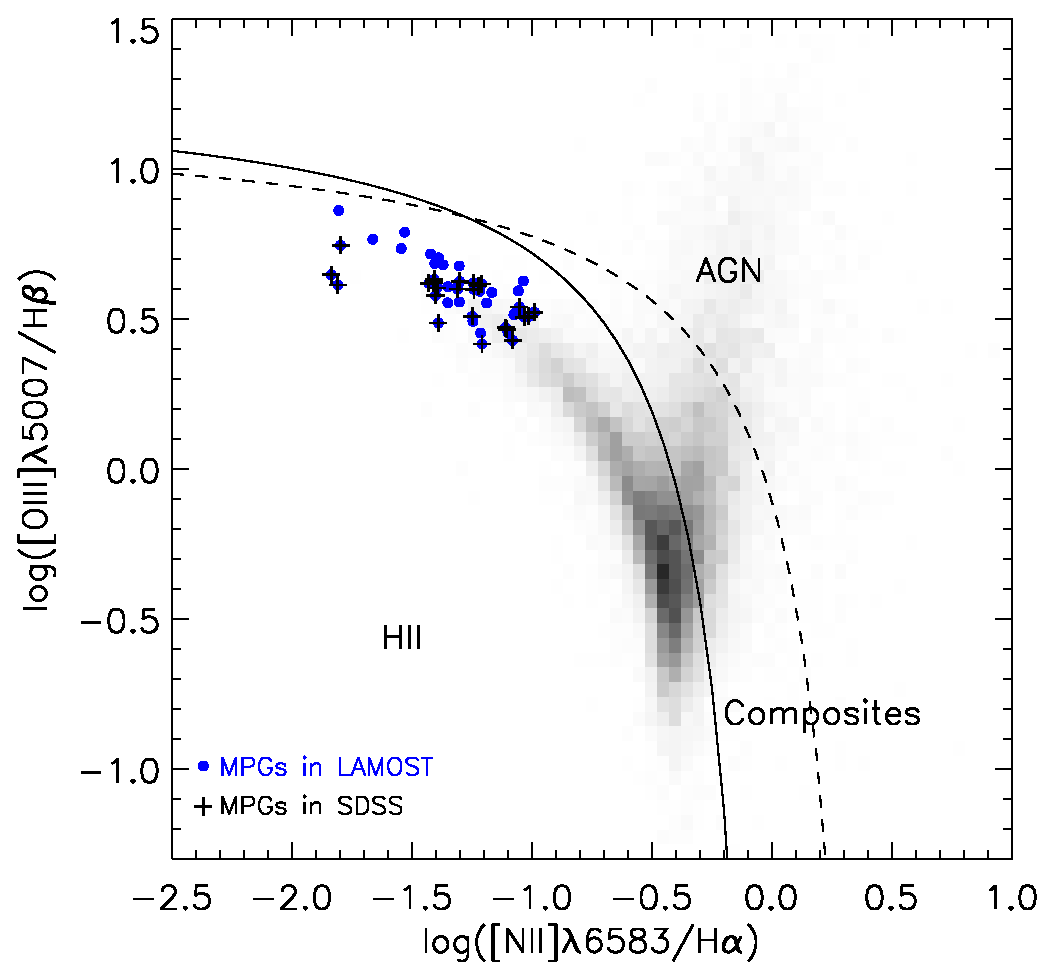
\includegraphics[width=3.5in]{fig2}
\caption{Decomposition of some complicated quantum gates.}
\label{fig2}
\end{figure}

Based on the foregoing, it is clear that the implementation of transform $\mathcal{H}$ in Step 1 requires $l$ Hadamard gates to execute. In addition, transform $\mathcal{R}$ in Step 2 can be divided into $2^l$ sub-operations (i.e. $R_t$) to store the amplitude information for each sample. Therefore, with the assistance of enough ancillary qubits, each sub-operation $R_t$ can be directly implemented using $2\left( l - 1 \right)$ Toffoli gates and no more than $q$ CNOT gates. Hence, the complexity of preparing a $2^l$-sized FRQA state is:
\begin{equation}\label{eq14}
2^l \times \left[ 2(l - 1) \times 6 + q \right] = \left( 12l + q - 12\right) \cdot 2^l,
\end{equation}
which indicates the efficiency of the preparation process. In order to further illustrate the complexity of constructing an FRQA quantum audio, we select the initialization of the sample at $\vert 0110\rangle$ in Fig. \ref{fig1} as an example. The network for implementing the operation, i.e. $R_6$ [when \emph{k} = 6 in Eq. (\ref{eq11})], is depicted in Fig. \ref{fig3}.

\begin{figure}[!t]
\centering
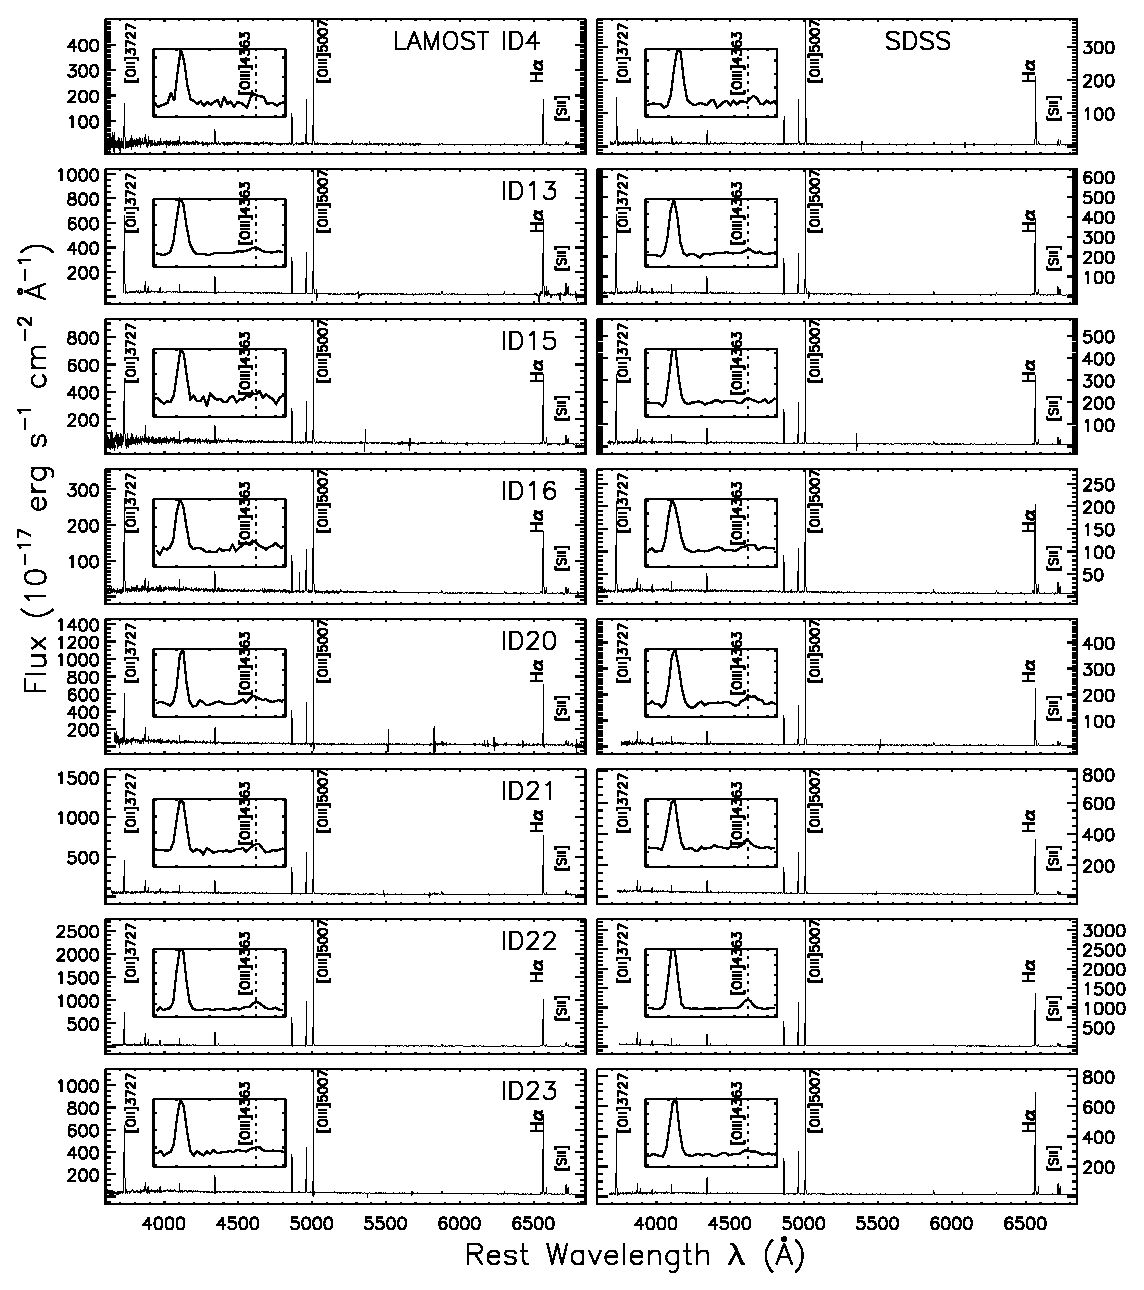
\includegraphics[width=3.5in]{fig3}
\caption{Network of implementing the $R_6$ operation when preparing the sample at $\vert 0110\rangle$ of FRQA state in Fig. \ref{fig1}.}
\label{fig3}
\end{figure}

\subsection{FRQA retrieval}\label{sec2-3}
The essential requirements for representing a quantum audio are the simplicity and efficiency in the storage and retrieval of the audio information. The storage of an FRQA audio is achieved by the preparation process as discussed in the preceding subsection. In this subsection, the rudiments required for the FRQA signal retrieval will be formalised.

Quantum measurement is the unique way of recovering classical information from a quantum state. To retrieve the amplitude information of each sample, quantum measurements $\Gamma$ and $M$ as defined in Eqs. (\ref{eq15}) and (\ref{eq16}) are used:
\begin{equation}\label{eq15}
\Gamma = {\sum_{t = 0}^{2^l - 1}} I^{\otimes q} \otimes {\vert t \rangle} {\langle t \vert},
\end{equation}
\begin{equation}\label{eq16}
M = {\sum_{m = 0}^{2^q - 1}} m {\vert m \rangle} {\langle m \vert}.
\end{equation}

Firstly, executing the quantum measurement operation $\Gamma$ on the time sequence extracts corresponding information of sample $t$ as $\vert P_t \rangle$, which is shown in Eq. (\ref{eq17}):
\begin{equation}\label{eq17}
\vert P_t \rangle = {\vert S_t \rangle} {\vert t \rangle},
\end{equation}
and then, the projective measurement $M$ is used to recover the amplitude value from the quantum state:
\begin{equation}\label{eq18}
\begin{aligned}
{\langle S_t \vert} M {\vert S_t \rangle} & = {\langle S_t \vert} \left( {{\sum_{m = 0}^{2^q - 1}} m {\vert m \rangle} {\langle m \vert}} \right) {\vert S_t \rangle} \\
& = {\sum_{m = 0}^{2^q - 1}} m {\langle S_t \vert} {\vert m \rangle} {\langle m \vert} {\vert S_t \rangle} = S_t.
\end{aligned}
\end{equation}

Through these measurement operations, the amplitude value of sample $k$ will be recovered. This means that all the samples in a quantum audio signal can be recovered in the same way, so the original digital audio can be retrieved from the FRQA state (Note that it is the theoretical discussion about the quantum information retrieval. We will not touch at all on the consequence of decoherence or any errors appeared in the process.)

\section{Operations on quantum audio signals}\label{sec3}
Basic signal operations are the foundations of digital audio processing. The ability to extend similar operations to quantum audio processing is essential to validating the utility of this emerging sub-field of quantum information processing. In this section, we will present a few basic audio signal operations including signal addition, signal inversion, signal delay, and signal reversal based on the FRQA representation.

\subsection{Signal addition}\label{sec3-1}
Signal addition is among the fundamental operations in audio signal processing. This operation involves the addition of amplitudes of two or more signals at each instant of time. By means of this operation, a series of audio signal processing like echo or reverb addition and active noise reduction can be implemented. Representing the amplitude values in two's complement system in FRQA facilitates determining the results of the arithmetic operations and depicting the waveform with respect to the midrange. Hence, we can define the signal addition operation based on this arithmetic advantage as below.

Assuming that $\vert A_x \rangle$ and $\vert A_y \rangle$ are two $2^l$ audio segments as presented in Eqs. (\ref{eq19})-(\ref{eq20}), the signal addition operation produces the output of $\vert A_z \rangle$ as shown in Eq. (\ref{eq21}):
\begin{equation}\label{eq19}
\vert A_x \rangle = {1\over 2^{l/2}}{\sum_{x=0}^{2^{l} - 1}{\vert S_x\rangle}\otimes \vert t_x\rangle}, \notag
\end{equation}
where
\begin{equation}
\vert t_x \rangle = \vert t_x^0t_x^1\ldots t_x^{l-1} \rangle, t_x^i\in\{0, 1\}, \notag
\end{equation}
\begin{equation}
\vert S_x \rangle = \vert S_x^0S_x^1\ldots S_x^{q-1} \rangle, S_x^i \in\{0, 1\},
\end{equation}
and
\begin{equation}\label{eq20}
\vert A_y \rangle = {1\over 2^{l/2}}{\sum_{y=0}^{2^{l} - 1}{\vert S_y\rangle}\otimes \vert t_y\rangle}, \notag
\end{equation}
where
\begin{equation}
\vert t_y \rangle = \vert t_y^0t_y^1\ldots t_y^{l-1} \rangle, t_y^i\in\{0, 1\}, \notag
\end{equation}
\begin{equation}
\vert S_y \rangle = \vert S_y^0S_y^1\ldots S_y^{q-1} \rangle, S_y^i \in\{0, 1\},
\end{equation}
so
\begin{equation}\label{eq21}
\vert A_z \rangle = {1\over 2^{l/2}}{\sum_{z=0}^{2^{l} - 1}{\vert S_z\rangle}\otimes \vert t_z\rangle}, \notag
\end{equation}
where
\begin{equation}
\vert t_z \rangle = \vert t_z^0t_z^1\ldots t_z^{l-1} \rangle, t_z^i\in\{0, 1\}, \notag
\end{equation}
\begin{equation}
\vert S_z \rangle = \vert S_z^0S_z^1\ldots S_z^{q}\rangle = \vert S_x + S_y \rangle, S_z^i \in\{0, 1\}, \notag
\end{equation}
\begin{equation}
t_z = t_x = t_y.
\end{equation}

Quantum algorithms are tools for constructing advanced operations using circuit elements. In order to construct the quantum circuit to execute the signal addition operation, we start by introducing two commonly-used quantum modules that are presented in Fig. \ref{fig4}.

\begin{figure}[!t]
\centering
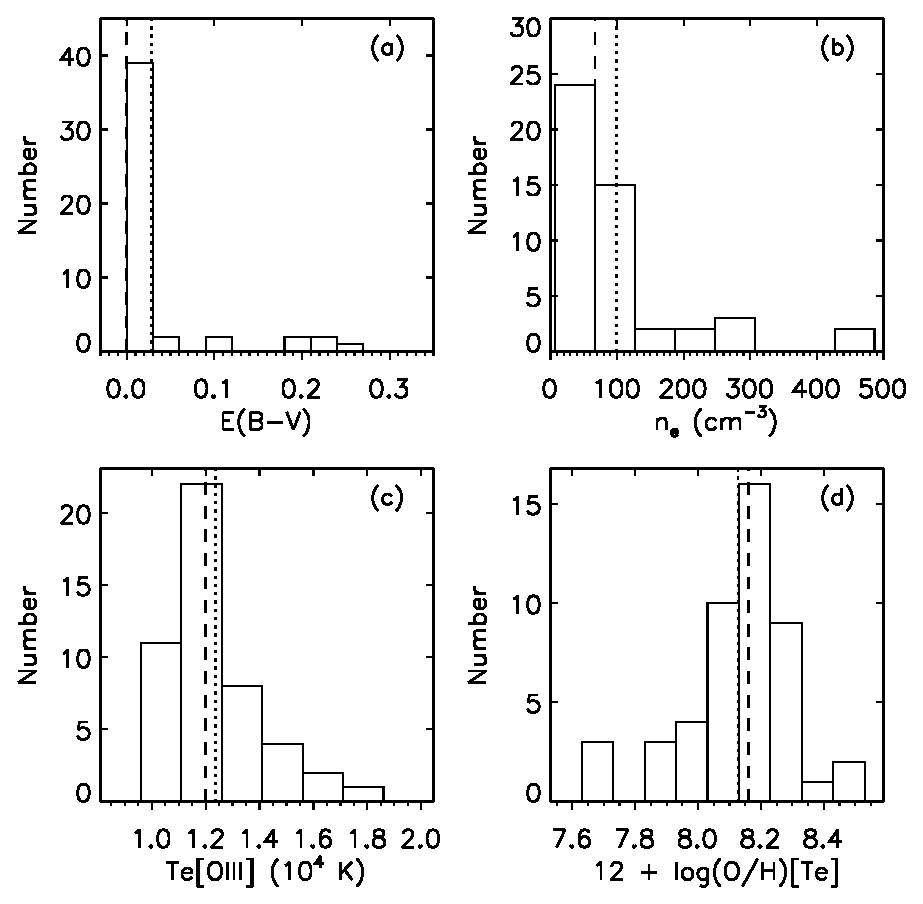
\includegraphics[width=3in]{fig4}
\caption{(a) The quantum ADDER module and (b) the quantum comparator module.}
\label{fig4}
\end{figure}

The ADDER module \cite{13} is designed to realize the operation $\vert a \rangle\vert b \rangle \rightarrow \vert a \rangle\vert a + b \rangle$, where $\vert a \rangle$ and $\vert b \rangle$ are two quantum sequences both with $q$ qubits, and $\vert a + b \rangle$ = $\vert d_0d_1\ldots d_{q} \rangle$ is a quantum sequence with $(q + 1)$ qubits that represents the result of addition. By using the ADDER module and necessary control conditions, we can realize the addition of amplitude values in two segments of quantum audio at any given instant of time.

The other module presented in Fig. \ref{fig4} is the quantum comparator module \cite{15} that is used to compare two $l$-qubit binary sequences ($\vert a\rangle$ and $\vert b\rangle$) and stores the result in the ancilla qubits $\vert e_0e_1 \rangle$. A useful output of $\vert e_0e_1 \rangle$ in this study is when $\vert e_0e_1 \rangle = \vert 00 \rangle$, then $\vert a\rangle = \vert b\rangle$. The comparator module guarantees that the two operands in the addition are the amplitude values of the two audio segments at the same instant of time.

Hence, the operation of FRQA-based signal addition operation $\mathcal{U}_A$ can be written in the form:

\begin{equation}\label{eq22}
\mathcal{U}_A : \vert S_x \rangle\vert S_y \rangle \rightarrow \vert S_x \rangle\vert S_x + S_y \rangle.
\end{equation}

The quantum circuit to realize the operation $\mathcal{U}_A$ is depicted in Fig. \ref{fig5}, where the ADDER operation is applied on the amplitude content and the comparator operation is applied on the time content. Additionally, in order to avoid the overflow during two's complement addition, we design a sign extension module (denoted as ``EXT" in Fig. \ref{fig5}) which helps to increase the length of the binary sequence while preserving the sign information in the ADDER module. To conclude our discussion of the signal addition operation, an example for the case when $l = 2$ and $q = 2$ is presented in Fig. \ref{fig6}.

As seen in Fig. \ref{fig5}, the circuit network for implementing the signal addition operation is divided into 3 parts: a comparator module, a $2$-controlled ``EXT" module, and a $2$-controlled ADDER module. Implementations of the ADDER and comparator module have been extensively discussed in \cite{15} and \cite{16}. Additionally, the computational complexities of the two modules are $28q - 12$ and $24l^2 + 6l$, respectively, where $q$ and $l$ denote the length of the inputs as shown in Fig. \ref{fig4}. Consequently, to effectively quantify the complexity of the operation $\mathcal{U}_A$ depicted in Fig. \ref{fig5}, we only need to determine the complexity of the $2$-controlled ``EXT" module and $2$-controlled ADDER module.

The $2$-controlled ``EXT" module is a pair of $4$-controlled NOT gates, so complexity of this part is $ 2 \times [2 \times (4-1) \times 6 + 1] = 74$. The ADDER module consists of $4q-2$ Toffoli gates and $4q$ CNOT gates \cite{16}, so the $2$-controlled unit consists of $\underline{4q-2}$ $4$-controlled NOT gates and $4q$ $3$-controlled NOT gates, thereby the complexity of this controlled module is $248q - 74$. Based on these analyses, the complexity of the entire signal addition operation is $24l^2 + 6l + 248q$.

\begin{figure}[!t]
\centering
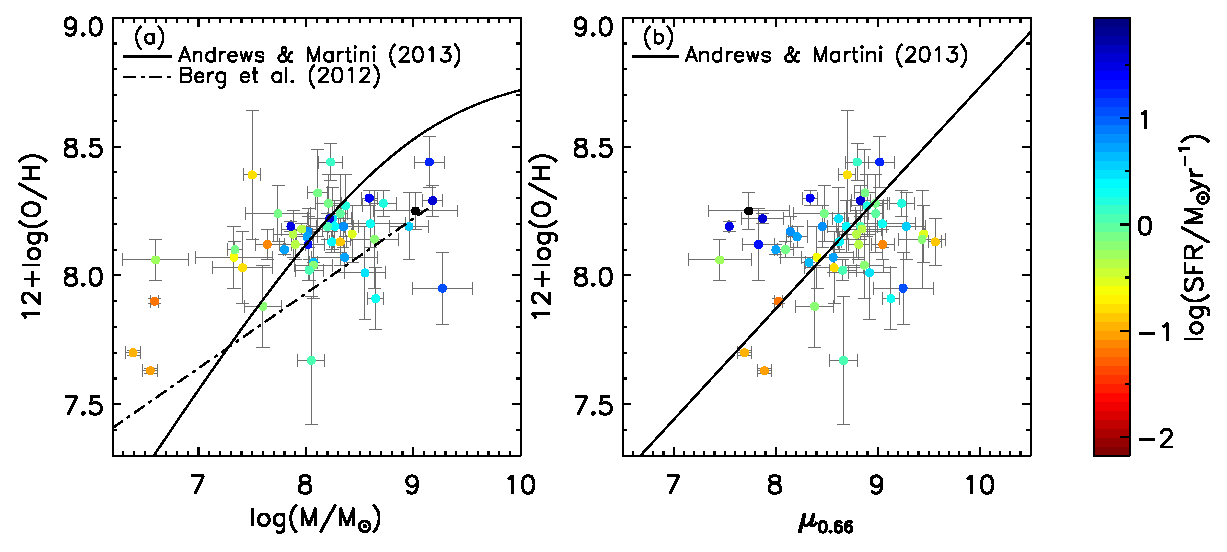
\includegraphics[width=3.2in]{fig5}
\caption{Circuit construction to execute the quantum audio signal addition operation.}
\label{fig5}
\end{figure}
\begin{figure}[!t]
\centering
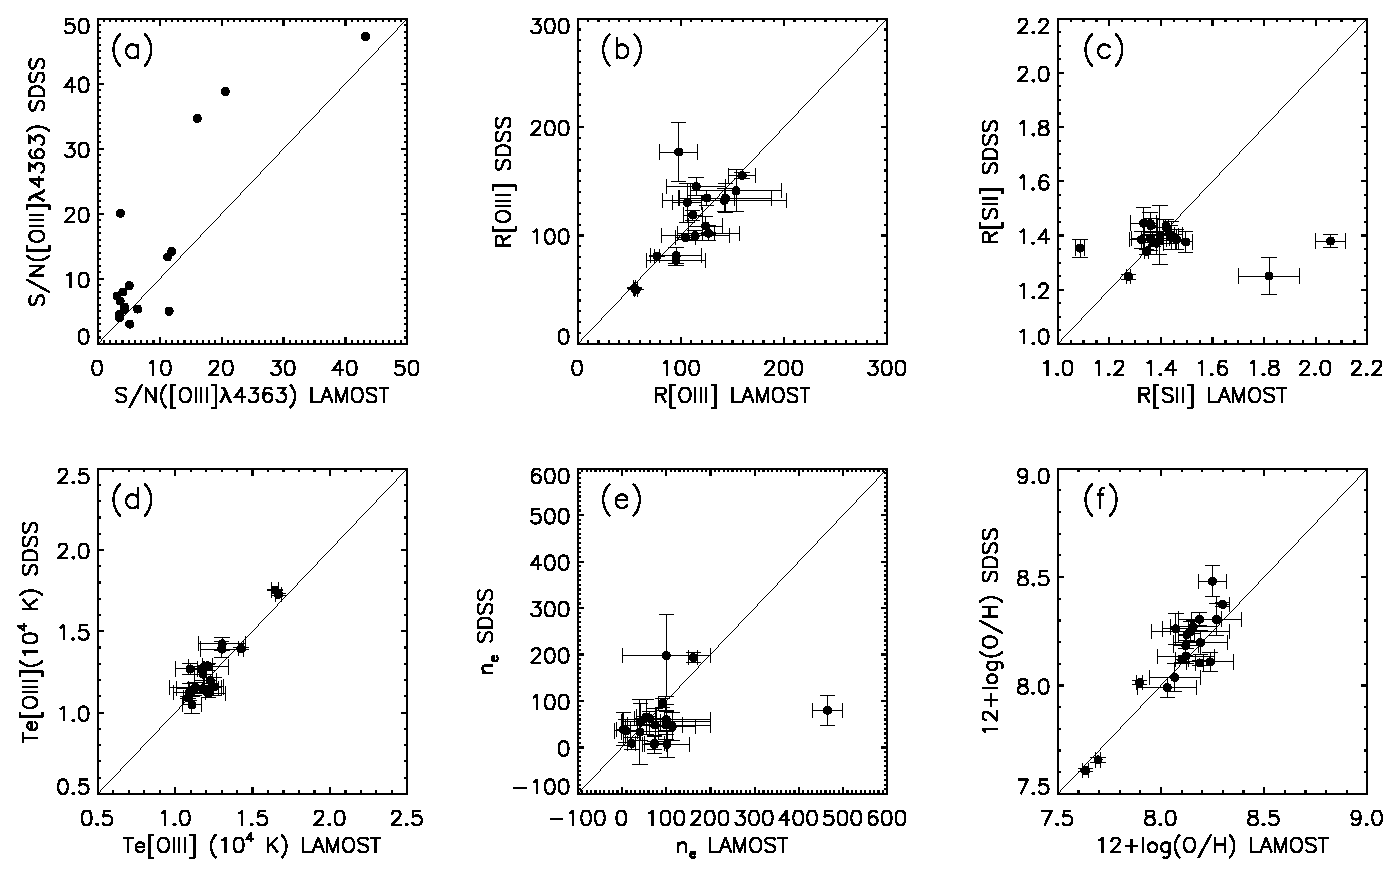
\includegraphics[width=3.5in]{fig6}
\caption{An example of quantum audio signal addition operation.}
\label{fig6}
\end{figure}

\subsection{Signal inversion}\label{sec3-2}
Inverting a signal is common in signal processing algorithms. A meaningful usage of inversion is to transform the signal subtraction to signal addition by means of inverted inputs (audio cancellation is realized as so). In audio signal processing, signal inversion is realized by inverting all amplitude values of an audio signal. When amplitude values are represented by bipolar values, the operation is essentially an alteration of positive and negative signs. In this subsection, the FRQA-based signal inversion operation is formalised.

Assuming that $\vert A \rangle$ is an FRQA audio in the form presented in Eq. (\ref{eq3}), the signal inversion operation $\mathcal{U}_I$ applied on $\vert A \rangle$ will produce the output of $\vert A_I \rangle$ in the form shown in Eq. (\ref{eq23}):
\begin{equation}\label{eq23}
\vert A_I \rangle = {1\over 2^{l/2}}{\sum_{t=0}^{2^{l} - 1}{\vert S_I\rangle}\otimes \vert t\rangle}, \notag
\end{equation}
where
\begin{equation}
\vert t \rangle = \vert t_0t_1\ldots t_{l-1} \rangle, t_i\in\{0, 1\}, \notag
\end{equation}
\begin{equation}
\vert S_I \rangle = \vert - S_t^0S_t^1\ldots S_t^{q-1} \rangle = \vert - S_t \rangle, S_t^i \in\{0, 1\}.
\end{equation}

As in two's complement arithmetic, an effective way to negate a number is inverting all the qubits and adding ``1''. This procedure in quantum audio processing is further explained using the following steps:

\textbf{Step 1:} Invert all the qubits in $\vert S_t\rangle$ by performing operation $\mathcal{U}_{I}^1$:
\begin{equation}\label{eq24}
\begin{aligned}
\mathcal{U}_{I}^1(\vert A\rangle) & = {1\over 2^{l/2}}{\mathcal{U}_{I}^1(\sum_{t=0}^{2^{l} - 1}{\vert S_t\rangle})\otimes \vert t\rangle} \\
& = {1\over 2^{l/2}}{\sum_{t=0}^{2^{l} - 1}{\vert \overline{S_t}\rangle}\otimes \vert t\rangle}, \notag
\end{aligned}
\end{equation}
where
\begin{equation}
\vert S_t \rangle = \vert S_t^0S_t^1\ldots S_t^{q-1} \rangle, S_t^i \in\{0, 1\}, \notag
\end{equation}
\begin{equation}
\vert \overline{S_t} \rangle = \vert \overline{S_t^0 S_t^1 \ldots S_t^{q-1}} \rangle, \overline{S_t^i} \in\{0, 1\}.
\end{equation}

\textbf{Step 2:} Add ``1'' to the inverted result $\vert \overline{S_t}\rangle$ and neglect the overflow by applying operation $\mathcal{U}_{I}^2$:
\begin{equation}\label{eq25}
\mathcal{U}_{I}^2 : \vert \overline{S_t} \rangle \rightarrow = \vert S_I \rangle, \notag
\end{equation}
where
\begin{equation}
\vert \overline{S_t} \rangle = \vert \overline{S_t^0 S_t^1 \ldots S_t^{q-1}} \rangle, \notag
\end{equation}
\begin{equation}
\vert (\overline{S_t^0 S_t^1 \ldots S_t^{q-1}} + 1) \bmod 2^{q} \rangle = \vert S_I \rangle.
\end{equation}

It should be noted that similar to what is obtained in (classical) digital audio signal processing, a slight skewing of the data range is unavoidable as we cannot find the inverted counterpart of $\vert -2^{q-1}\rangle$ in the sampled amplitude values $s_t$. To overcome this, we restrict our discussion within the amplitude value range from $\vert -2^{q-1} + 1\rangle$ to $\vert 2^{q-1} - 1\rangle$. The quantum circuit for inverting an FRQA audio signal is shown in Fig. \ref{fig7}, wherein, the operation $\mathcal{U}_{I}^1$ in Step 1 can be directly implemented by using $q$ NOT gates and in the operation $\mathcal{U}_{I}^2$ in Step 2, $q - 1$ Toffoli gates and $q$ CNOT gates are required, thus the complexity of this operation is $7q - 6$.

A simple example to illustrate how a quantum audio signal is inverted would suffice. The circuit network required to execute this procedure is presented in Fig. \ref{fig8}, where the FRQA audio $\vert A_z\rangle$ in Fig. \ref{fig6} is used as the input audio signal.

\begin{figure}[!t]
\centering
\includegraphics[width=3in]{fig7}
\caption{Circuit construction to execute the quantum audio signal inversion operation.}
\label{fig7}
\end{figure}

\begin{figure}[!t]
\centering
\includegraphics[width=3.4in]{fig8}
\caption{An example of the quantum audio signal inversion operation ($\vert A_I\rangle$ is the inverted version of $\vert A_z\rangle$ in Fig. \ref{fig6}).}
\label{fig8}
\end{figure}

\subsection{Signal delay}\label{sec3-3}
Signal delay is the operation that records an input signal and then plays it back after a period of time. This operation is a common audio effect that is often used to create the sound of a repeating and decaying echo. In this subsection, the FRQA-based signal delay operation is formalised.

Assuming $A(t)$ is the original audio signal, then audio signal $B(t)$ is regarded as a delayed version of audio $A(t)$ if:

\begin{equation}\label{eq26}
A(t) = B(t^{\prime}), t^{\prime} = t + \triangle{t},
\end{equation}
where $t$ denotes the time information of amplitude values, $\triangle{t}$ is a fixed interval which specifies the desired delay of the system. Using the foregoing, the signal delay operation $\mathcal{U}_D$ can be described using Eqs. (\ref{eq27})-(\ref{eq28}):

\begin{equation}\label{eq27}
\mathcal{U}_{D} : A(t) \rightarrow B(t^{\prime}), t^{\prime} = t + \triangle{t},
\end{equation}
\begin{equation}\label{eq28}
B(t^{\prime}) = \left \{ \begin{array}{ll}
0 , & 0 \leq t^{\prime} \leq \triangle{t-1}\\
A(t) , & \triangle{t} \leq t^{\prime} \leq 2^{l}-1\\
\end{array}\right..
\end{equation}

Both the time information $t$ and $t^{\prime}$ of the original and delayed audio signal need to be in the range $[0, 2^l - 1]$, where apparently $\triangle{t} \leq t^{\prime} = t + \triangle{t} \leq 2^l + \triangle{t} - 1$ is beyond the interval. Therefore, we separate the time information into two parts, i.e. $[\triangle{t}, 2^l - 1]$ and $[2^l, 2^l + \triangle{t} - 1]$, for discussion.

As shown in Eq. (\ref{eq28}), when $t^{\prime} \in [\triangle{t}, 2^l - 1]$, $B(t^{\prime}) = A(t)$, in which case, the time information $t^{\prime}$ can be obtained directly by means of the ADDER module on time content. However, when $t^{\prime} \in [2^l, 2^l + \triangle{t} - 1]$, we need to employ the carry qubit of the ADDER module to achieve the interval shift $[2^l, 2^l + \triangle{t} - 1] - 2^l = [0, \triangle{t}-1]$ and set the amplitudes $S_t = 0$ as the delay period.

The general circuit for the quantum audio signal delay operation is presented in Fig. \ref{fig9}. In addition, Fig. \ref{fig10} presents a simple example of the FRQA-based signal delay, where (a) is the input audio signal ($l = 3$ and $q = 3$) and (b) is the signal that is delayed by 2 time units. The quantum circuit for this operation can be constructed as in Fig. \ref{fig11}.

The implementation of signal delay consists of one ADDER module (on time content) and $2q$ Toffoli gates, so the complexity of this operation is $28l + 12q - 12$.

\begin{figure}[!t]
\centering
\includegraphics[width=3.1in]{fig9}
\caption{General circuit for quantum audio signal delay operation.}
\label{fig9}
\end{figure}

\begin{figure}[!t]
\centering
\includegraphics[width=3.5in]{fig10}
\caption{(a) The input quantum audio signal and (b) the delayed signal.}
\label{fig10}
\end{figure}

\begin{figure}[!t]
\centering
\includegraphics[width=3.5in]{fig11}
\caption{Circuit construction to execute the quantum audio signal delay example in Fig. \ref{fig10}.}
\label{fig11}
\end{figure}

\subsection{Signal reversal}\label{sec3-4}
Signal reversal is the process of reversing a selected audio signal such that the end of the signal is heard first and the beginning last. This operation can be used to create interesting sound effects or make small portions of inappropriate language unintelligible. Based on the FRQA state, we can define the signal reversal operation on quantum computers and construct the quantum circuit to accomplish it.

Assuming that $\vert A\rangle$ is an FRQA audio signal in the form presented in Eq. (\ref{eq3}), the signal reversal operation $\mathcal{U}_R$ applied on $\vert A \rangle$ produces an output of the form:

\begin{equation}\label{eq29}
\vert A_R \rangle = {1\over 2^{l/2}}{\sum_{t=0}^{2^{l} - 1}{\vert S_t\rangle}\otimes \vert \overline{t}\rangle}, \notag
\end{equation}
where
\begin{equation}
\vert \overline{t} \rangle = \vert \overline{t_0t_1\ldots t_{l-1}} \rangle, \overline{t_i}\in\{0, 1\}.
\end{equation}

Hence, the signal reversal operation $\mathcal{U}_R$ can be defined as below:

\begin{equation}\label{eq30}
\begin{aligned}
\mathcal{U}_R(\vert A \rangle)& = {1\over 2^{l/2}}{\sum_{t=0}^{2^{l} - 1}{\vert S_t\rangle}\otimes \mathcal{U}_R(\vert t\rangle)} \\
& = {1\over 2^{l/2}}{\sum_{t=0}^{2^{l} - 1}{\vert S_t\rangle}\otimes \vert \overline{t}\rangle}.
\end{aligned}
\end{equation}

The general circuit to execute the signal reversal operation is presented in Fig. \ref{fig12}(a). Although it is glaring that this operation can be directly implemented by using $l$ NOT gates, in order to further enunciate its realization, we use the quantum audio signal in Fig. \ref{fig10}(a) as input signal whose output is presented in Fig. \ref{fig12}(b). As seen, the result shows that all the time points are played in a reversed order.

In addition, some control condition constraints on the time content will allow us to confine the execution of the reversal operation $\mathcal{U}_R$ to a desired period. For example, in Fig. \ref{fig13}(a), the time wire $t_0$ is employed as the control wire to confine the reversal operation to the last half of the audio signal. As seen from the result in Fig. \ref{fig13}(b) that only the last 4 time points in Fig. \ref{fig10}(a) are reversed and the others are retained as in the input signal.

It should be mentioned that the complexity of the extended operation increases with the number of control qubits. In the worst case, the implementation of this operation requires an $(l-1)$-controlled NOT gate, thereby the complexity is $12l - 23$.

\begin{figure}[!t]
\centering
\includegraphics[width=3.5in]{fig12}
\caption{(a) General circuit for quantum audio signal reversal and (b) a simple example of this operation.}
\label{fig12}
\end{figure}

\begin{figure}[!t]
\centering
\includegraphics[width=3.5in]{fig13}
\caption{(a) Circuit construction to execute the restricted quantum audio signal reversal and (b) a simple example of this operation.}
\label{fig13}
\end{figure}
% needed in second column of first page if using \IEEEpubid
%\IEEEpubidadjcol

%\subsubsection{Subsubsection Heading Here}
%Subsubsection text here.

% An example of a floating figure using the graphicx package.
% Note that \label must occur AFTER (or within) \caption.
% For figures, \caption should occur after the \includegraphics.
% Note that IEEEtran v1.7 and later has special internal code that
% is designed to preserve the operation of \label within \caption
% even when the captionsoff option is in effect. However, because
% of issues like this, it may be the safest practice to put all your
% \label just after \caption rather than within \caption{}.
%
% Reminder: the "draftcls" or "draftclsnofoot", not "draft", class
% option should be used if it is desired that the figures are to be
% displayed while in draft mode.
%
%\begin{figure}[!t]
%\centering
%\includegraphics[width=2.5in]{myfigure}
% where an .eps filename suffix will be assumed under latex,
% and a .pdf suffix will be assumed for pdflatex; or what has been declared
% via \DeclareGraphicsExtensions.
%\caption{Simulation results for the network.}
%\label{fig_sim}
%\end{figure}

% Note that the IEEE typically puts floats only at the top, even when this
% results in a large percentage of a column being occupied by floats.
% However, the Computer Society has been known to put floats at the bottom.

% An example of a double column floating figure using two subfigures.
% (The subfig.sty package must be loaded for this to work.)
% The subfigure \label commands are set within each subfloat command,
% and the \label for the overall figure must come after \caption.
% \hfil is used as a separator to get equal spacing.
% Watch out that the combined width of all the subfigures on a
% line do not exceed the text width or a line break will occur.
%
%\begin{figure*}[!t]
%\centering
%\subfloat[Case I]{\includegraphics[width=2.5in]{box}%
%\label{fig_first_case}}
%\hfil
%\subfloat[Case II]{\includegraphics[width=2.5in]{box}%
%\label{fig_second_case}}
%\caption{Simulation results for the network.}
%\label{fig_sim}
%\end{figure*}
%
% Note that often IEEE papers with subfigures do not employ subfigure
% captions (using the optional argument to \subfloat[]), but instead will
% reference/describe all of them (a), (b), etc., within the main caption.
% Be aware that for subfig.sty to generate the (a), (b), etc., subfigure
% labels, the optional argument to \subfloat must be present. If a
% subcaption is not desired, just leave its contents blank,
% e.g., \subfloat[].

% An example of a floating table. Note that, for IEEE style tables, the
% \caption command should come BEFORE the table and, given that table
% captions serve much like titles, are usually capitalized except for words
% such as a, an, and, as, at, but, by, for, in, nor, of, on, or, the, to
% and up, which are usually not capitalized unless they are the first or
% last word of the caption. Table text will default to \footnotesize as
% the IEEE normally uses this smaller font for tables.
% The \label must come after \caption as always.
%
%\begin{table}[!t]
%% increase table row spacing, adjust to taste
%\renewcommand{\arraystretch}{1.3}
% if using array.sty, it might be a good idea to tweak the value of
% \extrarowheight as needed to properly center the text within the cells
%\caption{An Example of a Table}
%\label{table_example}
%\centering
%% Some packages, such as MDW tools, offer better commands for making tables
%% than the plain LaTeX2e tabular which is used here.
%\begin{tabular}{|c||c|}
%\hline
%One & Two\\
%\hline
%Three & Four\\
%\hline
%\end{tabular}
%\end{table}

% Note that the IEEE does not put floats in the very first column
% - or typically anywhere on the first page for that matter. Also,
% in-text middle ("here") positioning is typically not used, but it
% is allowed and encouraged for Computer Society conferences (but
% not Computer Society journals). Most IEEE journals/conferences use
% top floats exclusively.
% Note that, LaTeX2e, unlike IEEE journals/conferences, places
% footnotes above bottom floats. This can be corrected via the
% \fnbelowfloat command of the stfloats package.

\section{Conclusions}\label{sec4}
The characteristics of the physical support used to embody information decide the power of a certain computational paradigm. Quantum computation has emerged as a powerful tool for efficient and secure information processing. As with any effort to process any type of information, the requirements for its encoding must be formalised. The study presented in this work explored the use of quantum mechanical properties that are at the core of quantum computers in order to encode, store, and manipulate audio signals. Inspired by the rudiments employed to capture digital audio signals, the first known effort to represent quantum audio signals (the QRDA) was broached. While QRDA extended audio processing into the quantum computing domain, its numerical representation of amplitude values only offers an encoding method for unipolar (i.e. non-negative) numbers so that its operations are susceptible to errors. The FRQA proposed in this study offers an accurate computation and extensive signal operations alternative to the QRDA. The FRQA protocol encodes amplitude values in two's complement notation so that the arithmetic advantages of doing so can be utilized to facilitate the construction of quantum circuits for amplitude transformations. By exploiting this, various operations that allow for designing advanced audio processing applications can be proposed.

Based on this new FRQA representation, basic manipulations targeting the amplitude and time components of the audio signals such as the quantum audio signal addition, inversion, reversal, and delay were formalised and insightful examples depicting their utility were also presented and discussed. The quantum circuits required to execute these basic operations on quantum audio signals were also presented and the computational requirements for their realization were analyzed.

In future work, the results from this study can be extended towards the following directions. First, considering the importance of basic operations in quantum audio processing, the operations presented in the study need to improved and new ones added to ensure the execution of more advanced algorithmic tasks. Secondly, the possibility of using quantum-based signal processing operations, such as quantum Fourier transformations \cite{14} and wavelet transformations \cite{17} which have proven well-studied in other quantum information processing applications to facilitate quantum audio manipulation needs to explored. Thirdly, the ``silent'' quantum movies proposed in \cite{18} provided impetus for the need of sound or audio on the quantum computing paradigm. A useful integration of movie strip (technically a collection of quantum images) with audio signal information will complete the quantum movie representation and facilitate more interesting applications. Finally, when the basic quantum audio signal operations are perfected, they could serve as the building block for the realization of more sophisticated algorithms used for particular applications such as watermarking, steganography, and encryption. These improvements will facilitate multimedia security during quantum information transmission.

% if have a single appendix:
%\appendix[Proof of the Zonklar Equations]
% or
%\appendix  % for no appendix heading
% do not use \section anymore after \appendix, only \section*
% is possibly needed

% use appendices with more than one appendix
% then use \section to start each appendix
% you must declare a \section before using any
% \subsection or using \label (\appendices by itself
% starts a section numbered zero.)
%
\
% use section* for acknowledgment
\ifCLASSOPTIONcompsoc
  % The Computer Society usually uses the plural form
  \section*{Acknowledgments}
  This work is supported by the National Natural Science Foundation of China (No. 61502053). Additionally, AMI acknowledges funding from the Prince Sattam Bin Abdulaziz University via the Deanship for Scientific Research Project Number 2016/01/6641.

\else
  % regular IEEE prefers the singular form
  \section*{Acknowledgment}
\fi

% Can use something like this to put references on a page
% by themselves when using endfloat and the captionsoff option.
\ifCLASSOPTIONcaptionsoff
  \newpage
\fi

% trigger a \newpage just before the given reference
% number - used to balance the columns on the last page
% adjust value as needed - may need to be readjusted if
% the document is modified later
%\IEEEtriggeratref{8}
% The "triggered" command can be changed if desired:
%\IEEEtriggercmd{\enlargethispage{-5in}}

% references section


\end{document}


